There are several different technologies which are applied in e-paper displays.
But since the developed prototype uses a screen, which uses a microencapsulated electrophoretic display, this section only describes this specific implementation.


\begin{figure}[h]
	\centering
	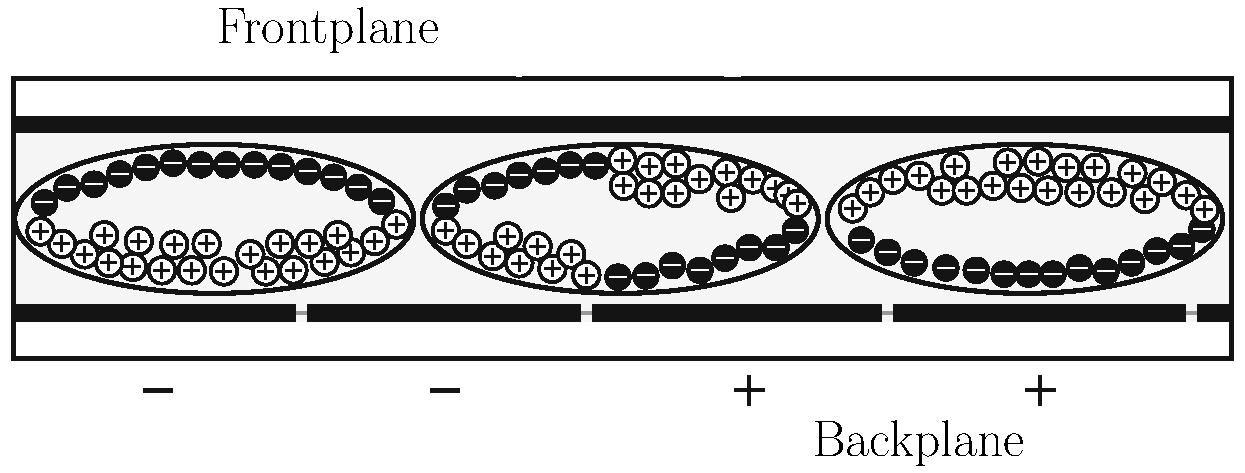
\includegraphics[width=0.9\textwidth]{2-theory/e-paper-display/graphics/capsules.png}
	\caption{filler pic\label{theory:capsules}}
\end{figure}

\begin{figure}[h]
	\centering
	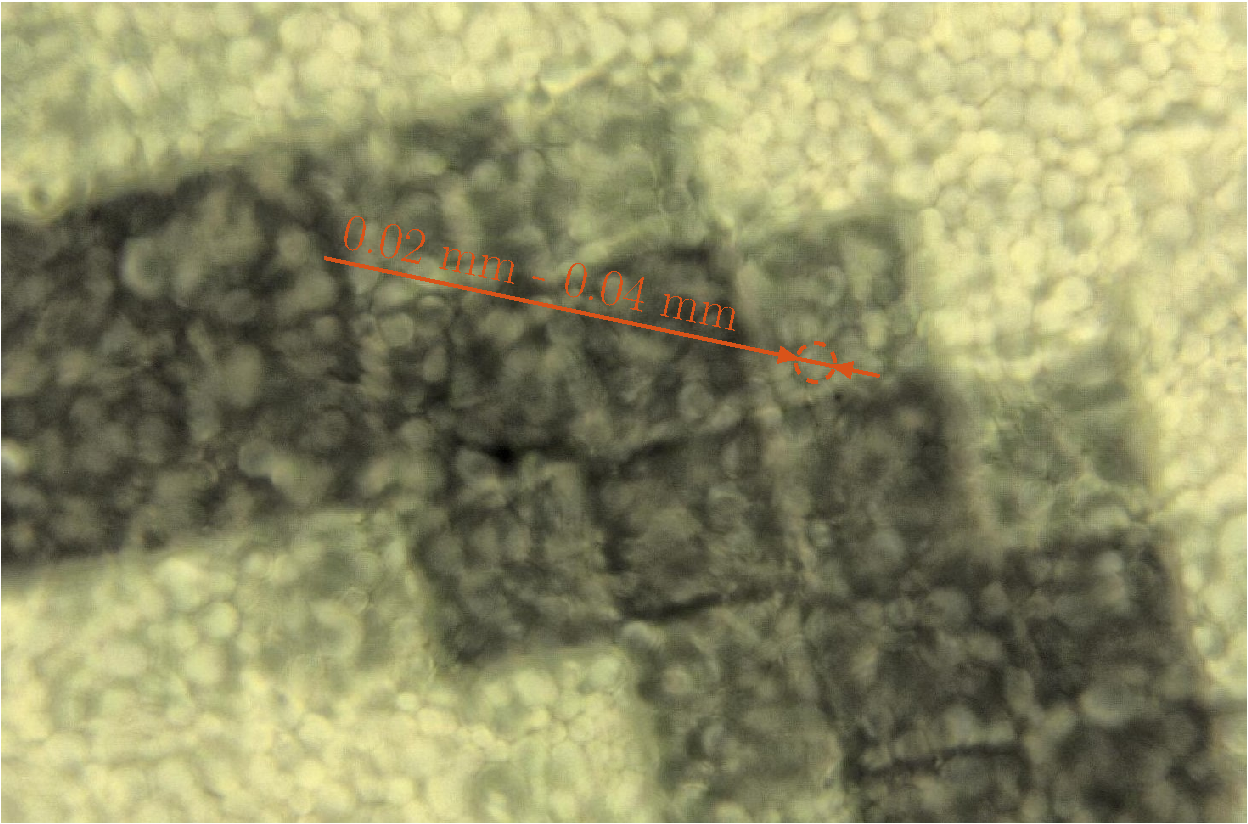
\includegraphics[width=0.9\textwidth]{2-theory/e-paper-display/graphics/epaper_mikroskop.pdf}
	\caption{E-paper display under microscope with 250x magnification\label{theory:micro}}
\end{figure}


\cite{amundson}